\section{Object Model}
\label{section:uml_notation}
\label{subsec:objects}

This section will cover the design choices behind the application's object model, derived from the use cases in Section~\ref{sec:use_cases}.
The UML object model diagram can be seen in Figure~\ref{fig:UML_class_diagram}, and is guided by the UML standard guide written by several different software companies in cooperation~\citep{UML_notation}.\\

The UML attribute notation in this report is:
\begin{itemize}
    \item PK attribute - means that the attribute is a primary key.
    \item FK attribute - means that the attribute is a foreign key.
    \item attribute : type - all attributes will have a type e.g. \verb+id : int+.
\end{itemize}

The system will contain the following objects: \deno{Affiliate Privilege}, \deno{Company}, \deno{Drone}, \deno{Privilege}, \deno{Role}, \deno{Session}, and \deno{User}.
The model of the objects and their relationships can be seen in Figure~\ref{fig:UML_class_diagram}.
Each object covered is represented in the object model diagram with its name in lowercase and pluralized, e.g. \deno{User} object $\rightarrow$ \deno{users}.
If an object's name consists of several words the spaces will be replaced by underscores, e.g. Session Key Task $\rightarrow$ session\_key\_tasks.

The relationship between two objects \deno{a} to \deno{b} can be either implicit or explicit.
Implicit relationships are illustrated as line from an \deno{a} to \deno{b}, where \deno{b} has a FK from \deno{a}
Explicit relationships can be either simple or rich.
Simple relationship models are models containing a FK from both \deno{a} and \deno{b} that is connected with a line to both.
They are represented in the model diagram with both objects in lowercase and pluralized, e.g. roles\_users.
Rich relationship models are similar to simple, but has a PK.
This kind of relationship model does not have a predetermined naming convention, therefore it can be anything as long as it does not collide with the other model names, e.g. user\_privileges.\\

\begin{figure}[htb]
    \centering
    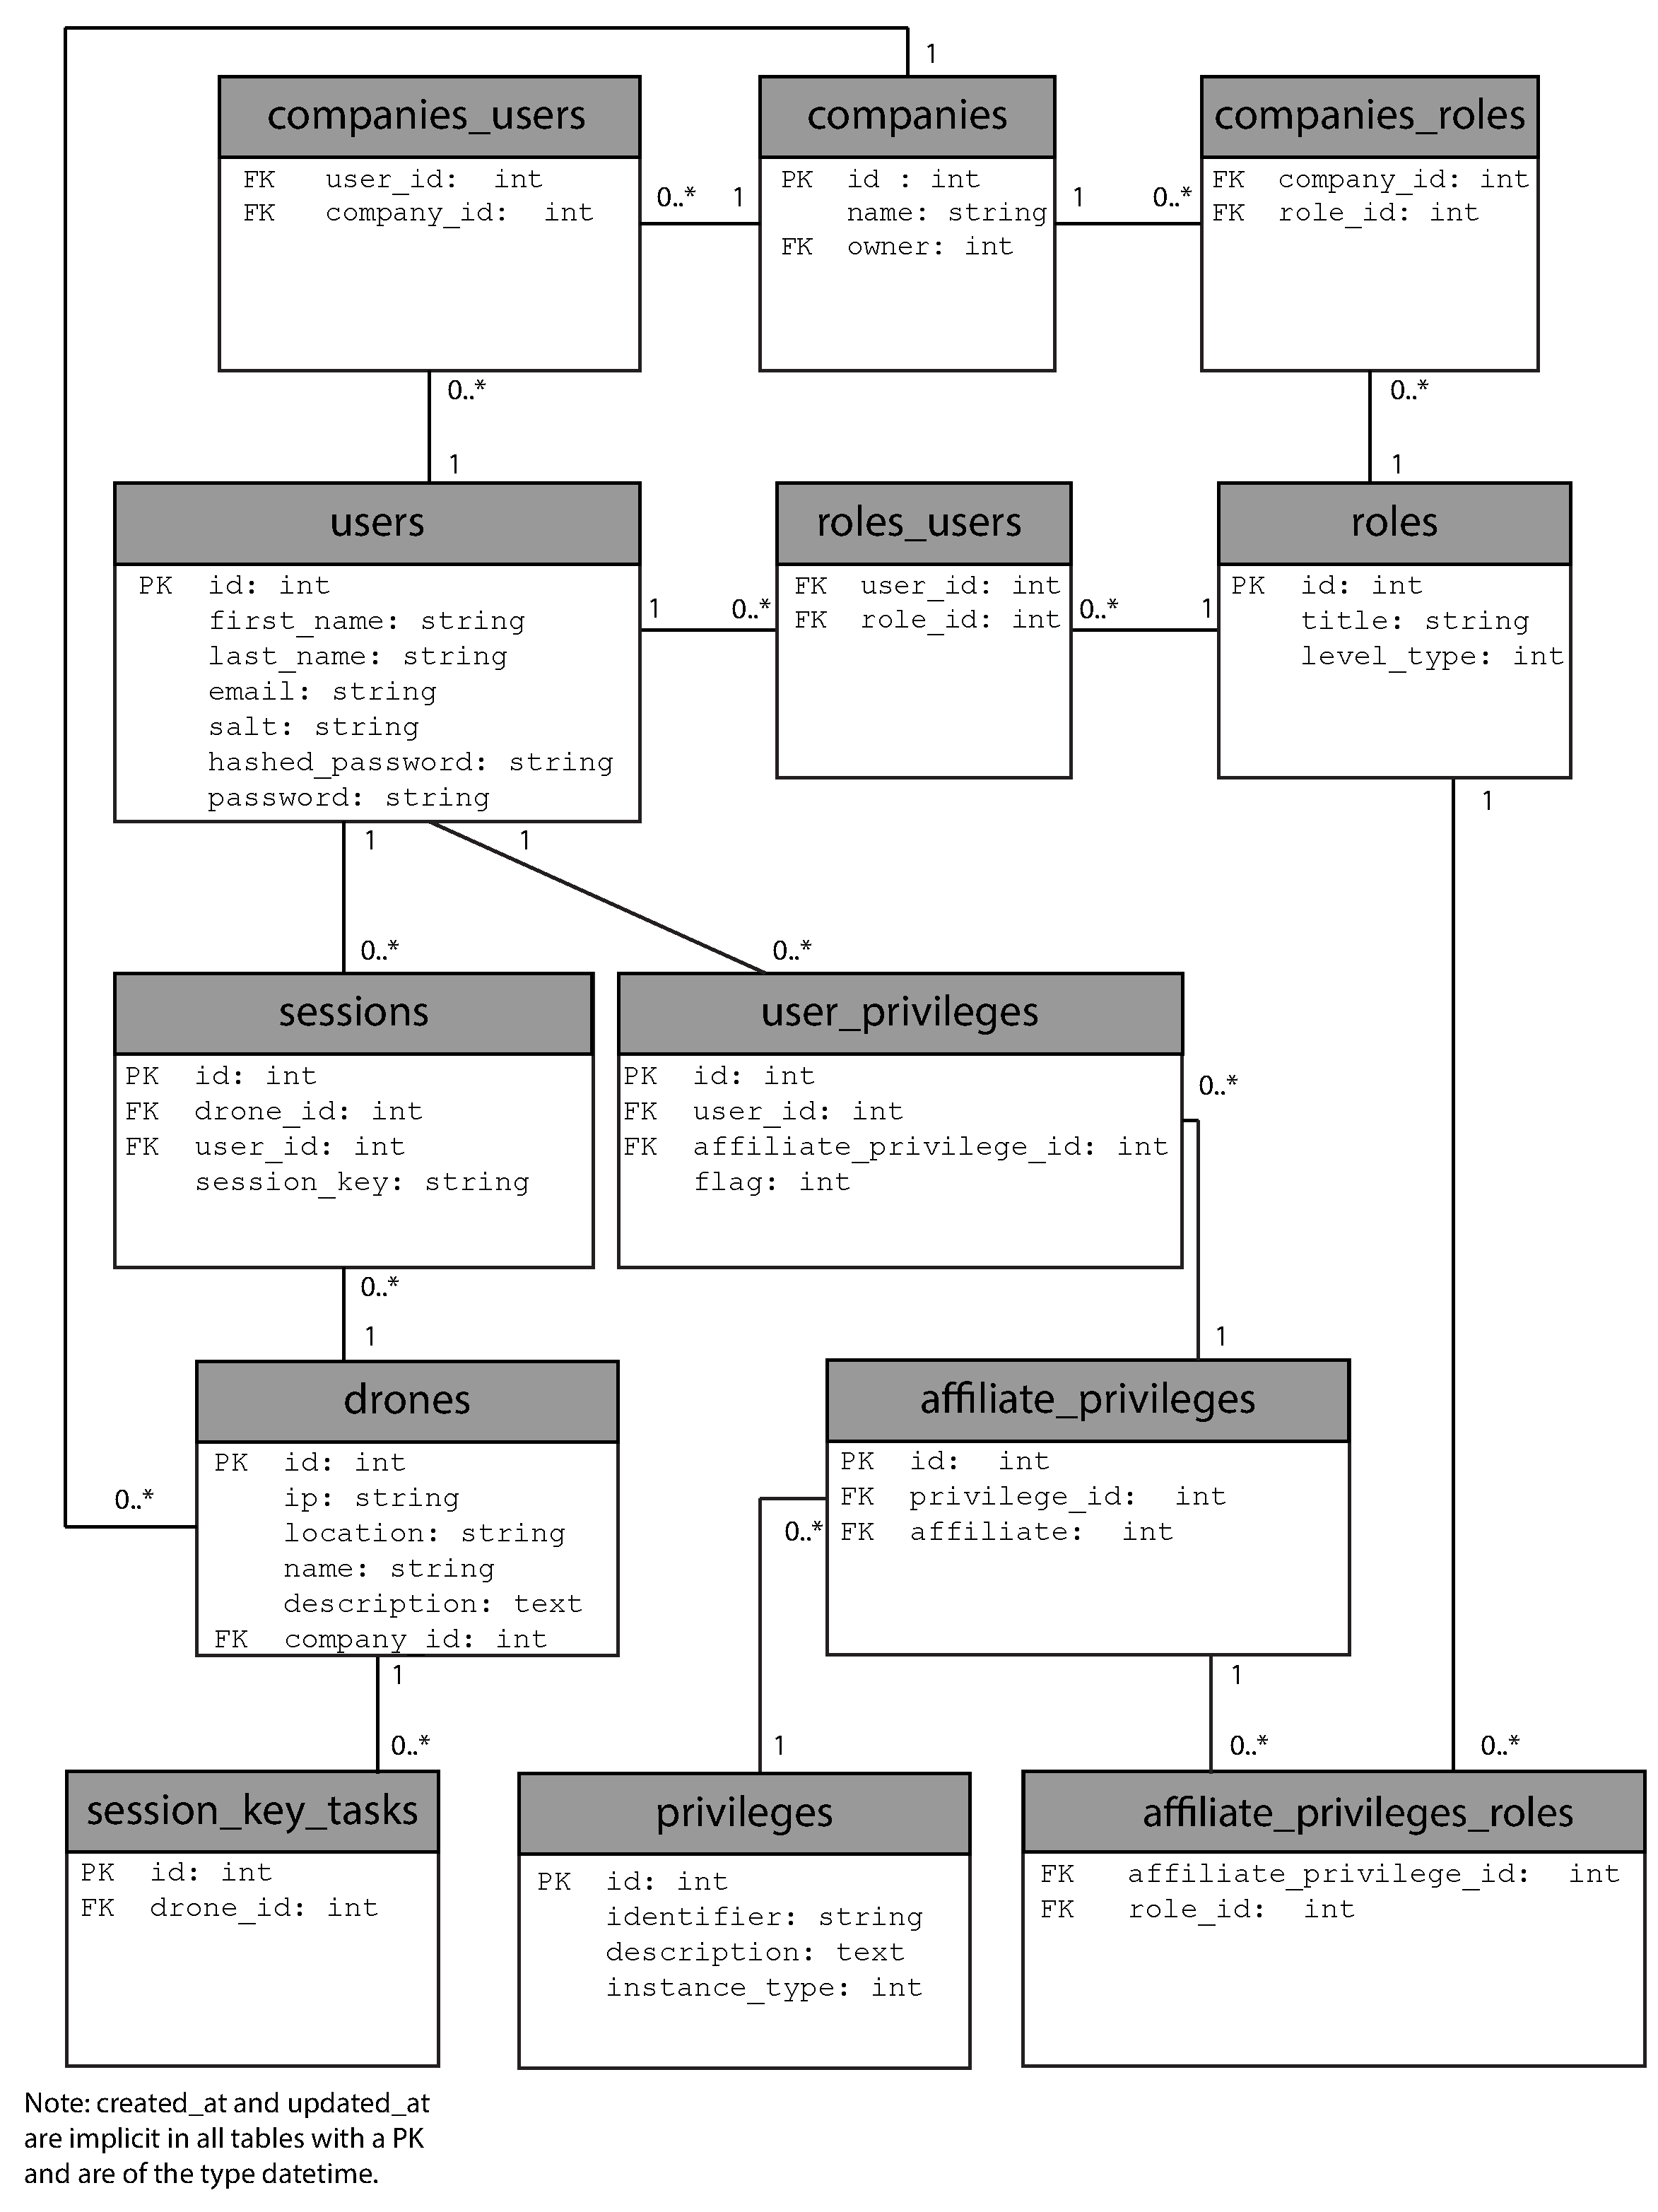
\includegraphics[width=0.95\textwidth]{gfx/UML_model.pdf}
    \caption{UML Class Diagram of \projectname{}.}
    \label{fig:UML_class_diagram}
\end{figure}


%\subsection{Objects} %\fixme{Skal denne overskrift være der? Det burde ikke være nødvendigt at have den, men så skal teksten ændres lidt.}
Access to the system and its functionality is restricted.
This restriction is based on the identity of the user in the system.
An instance of the \deno{User} object represents a user of the system.
The \deno{User} object has the attributes \verb+email+ and \verb+password+, as seen in Figure~\ref{tab:user_object} in Appendix~\ref{app:objects}, these combined form the login credentials needed for a user to authenticate his identity towards the system. \\

The \verb+email+ is publicly available.
Therefore the \verb+password+ must be protected in order for users to protect their user in the system.
The \verb+password+ entered by the user is concatenated with a \verb+salt+ and hashed through a SHA-1 hashing algorithm to be stored in \verb+hashed_password+.
The hashing algorithm provides a way for storing the password without having its exact value.
Storing passwords of users unencrypted would allow a third party to login into the system should he gain access to the database.
When a salt is concatenated before hashing it makes it harder for the third party to gain the original passwords, e.g. through a rainbow table~\cite{rainbow}. \\

Having a distributed setup with multiple \deno{S}, each representing a \deno{Drone} object, means that the network locations of these need to be known in order to communicate.
The network location is stored in the \verb+ip+ field of the \deno{Drone} object, as shown in Figure~\ref{tab:drone_object} of Appendix~\ref{app:objects}.
The physical drone has a unique identifier known as \verb+name+, which makes the user able to identify a given drone. \\

The users of the system will be part of different companies, as described in Section~\ref{sec:use_cases}, therefore there is a need for grouping users by a company.
The \deno{Company} object has an \verb+owner+, which is a reference to a \deno{User} object.
This is required for the system to know which user has access to all \deno{Affiliate Privilege} objects of the company. \\

An \deno{Affiliate Privilege} object references a \deno{Privilege}, and combined they form a unique key.
This key is associated with a specific functionality in the system.
A user is granted access to the functionality by having a relation with the \deno{Affiliate Privilege} that is part of the key.
\deno{Role} objects give the possibility of grouping \deno{Privilege} objects together.
Each \deno{Company} have a related role which contains all privileges, of which the company have full control.
Full control of a privilege gives the right to grant or revoke it from users.
\deno{Affiliate Privilege} objects have a field \verb+affiliate+ that links the privilege to an object of the type declared by the referenced \deno{Privilege} object's \verb+instance_type+ field. \\

The \deno{Session} object represents an active control connection between a user and a drone.
The \verb+session_key+ field provides a key that needs to be sent along with the commands.
The \deno{Session Key Task} object is an object used for \deno{D} and \deno{M} to communicate through \deno{DB}, as shown in Figure~\ref{fig:daemon_structure} in Section~\ref{sec:application_structure}. \\

In Section~\ref{sec:privileges} solutions for handling privileges were discussed.
From this discussion it was decided to model a system capable of handling all proposed solutions to fit scenarios of the users.
The \deno{User Privileges} relationship allows for connecting individual {Privilege} objects to a \deno{User} object.
This is could be either granting or revoking, i.e. creating exceptions, the privilege.
The \verb+flag+ field represents a value of either 1 or -1; 1 is regarded as granted, and -1 is regarded as revoked.


% \subsection{Relationships}
% The system is designed with flexibility and scalability in mind, and the structure of Roles and Privileges are what provides those features.
% As described before there are two ways that a User can be granted a specific Privilege.
% These are by 1) getting the Privilege granted directly via the \verb+User_Privileges+ table or 2) by being a member of a Role that via the \verb+Privileges_Roles+ table that has one or more Privileges granted.
% These will be explained in details in the following subsections.


% % Users and Privileges %
% An administrator can grant a specific Privilege directly to a user via the \verb+User_Privileges+ table.
% This Privilege is then affiliated with an object -- usually a Drone.
% The Privilege could also be a system functionality, however, as described in Section~\ref{sec:privileges}. \\

% This relationship is also used for exceptions.
% In an example where five Users: U1, U2, U3, U4 and U5 are a member of a Role: R1, we may have a situation where U2 is not suppose to have access to a given Privilege P1 in R1.
% Then a User-specific Privilege is granted to U2 on P1, but with the ``exception''-flag marked.
% This is equal to blacklisting U2 from using Privilege P1, providing the system with a lot of flexibility, as even though a group of Users are granted a number of Privileges via a role, User-specific exceptions can be added to this setting. \\


% % Roles and Privileges %
% As mentioned before -- the reason that Roles can be used to assign Privileges to a User, is to make both the administration and data structure of Users and Privileges as simple and efficient as possible.
% By allowing exceptions, full flexibility is still possible. \\

% This is how the relationship between Roles and Privileges works: \\

% An administrator creates a Role.
% Lets call this Role ``Control Drone \#4''.
% A number of Privileges are assigned to this Role.
% It could be the following:

% \begin{itemize}
%     \item Watch the video feed from a specific drone
%     \item Control the movement of a specific drone
% \end{itemize}

% Those Privileges are then linked to this Role and to the Drone this concerns. \\

% Roles can be assigned with affiliation to both Users and Companies.
% Say a user \verb+U1+ needs access to Drone \#4.
% User U1 then needs to either have the Privileges directly granted or be a member of the role ``Control Drone \#4''.


% % Privileges and granting of Privileges %
% Since it is possible to grant Privileges both directly to a User and via a Role, the same Privilege can be used in more than one context.
% Therefore the \verb+Affiliation_Privileges+ table exists.
% This table links the granting of a Privilege with the actual Privilege and defines on which Object the Privilege applies.
% The reason for having this table and not just link the two granting-tables \verb+User_Privileges+ and \verb+Privileges_Roles+ directly to the \verb+Privileges+ table, is that we try to avoid redundant data by having the data in the \verb+Privileges+ and \verb+Affiliation_Privileges+ table make up one instance of a privilege together.
% This is then granted to a User or a Role, who can then use the Privilege. \\

% The system is designed so that any User can grant a Privilege he already has already been granted to another User if he is permitted to.
% This is controlled via a ``re-grantable'' flag which is set in either the \verb+User_Privileges+ table or the \verb+Privileges_Roles+ table.
% By marking this flag as ``true'', the User or Users that via a Role is granted the Privilege in question, can via an interface in the system re-grant the Privilege to other Users in the same Company.


% %Note: Alle brugere kan videregrante et privilege hvis de har tilladelse til det. Det er et flag som sætes i user_privileges og privileges_roles, som tillader alle der har dette privilegie til at videregrante det. Husk at beskrive hvordan et privilege og et affiliation privilege til sammen giver et grant-able privilegie


% % Privileges and Drones %
% With \projectname{} in its current form, most Privileges that are granted will have an connected with a Drone.
% Privileges and its a affiliations are linked in the \verb+Affiliation_Privileges+ table.
% This is also where Drones are linked to any granted privilege. \\

% As described earlier, Drones are the current object-type implemented in the system.
% However, the structure and model of the system allows for later expansion, connection new objects such as stationary cameras or any other type of object to the system.
% The \verb+Affiliation_Privileges+ has a third field named \verb+object_id+.
% This field links the Privilege, the granting of it and the Object that this granting is valid for. \\

% An example could be linking Privilege P1, User U1 and Drone D1.
% Say P1 is the privilege for watching the video feed of a drone.
% Then the user U1 will have access to watch the video feed of Drone D1.


% % Drones and Companies %
% The \verb+Company_drones+ table defines a relationship between a Drone and a Company.

% The administrator of each Company defines the Roles in that Company.
% In doing so, he defines which Privileges that are granted in every Role.
% These Privileges are linked to a (Drone)-object.
% The system must make sure that any Company administrator cannot link a Privilege with a Object that is not within his control. \\

% This relationship defines which Drones are available to each Company.
% When a Company administrator adds new Roles (and hence Privileges), he is only able to associate it with Drones that are connected to the Company in question.
